\section{Machine Learning}
\begin{itemize}
    \item Overview of ML paradigms (supervised, unsupervised, etc.)
    \item Typical ML tasks (classification, regression, time series, etc.)
    \item Challenges in selecting appropriate methods
    \item Existing guidelines or frameworks for method selection
\end{itemize}

\subsection{Machine Learning Paradigms and Tasks}

Machine learning algorithms can be broadly categorized according to the type 
of supervision they receive during training. 
\textcite{mitchell1997machine_learning} defines a learning algorithm as a 
computer program that improves its performance at some task through experience. 
Three main learning paradigms are commonly distinguished in the literature: 
supervised learning, unsupervised learning, and reinforcement learning 
\parencite{bishop2006pattern_recognition_machine_learning}
\parencite[Chapter~5]{Goodfellow-et-al-2016}
\parencite{sarker2021machine_learning_algorithms_real_world_applications_research_directions}.
The following sections outline each paradigm and introduce some common 
tasks.

In supervised learning, the training data consists of input vectors paired 
with corresponding target values. The two most common supervised tasks are 
classification, where the goal is to assign an input to one of a finite number 
of discrete categories, and regression, where the goal is to predict a continuous 
numerical value 
\parencite{bishop2006pattern_recognition_machine_learning}
\parencite[Chapter~5]{Goodfellow-et-al-2016}.

In unsupervised learning, no target values are provided. The algorithm must 
instead identify structure in the data directly 
\parencite{bishop2006pattern_recognition_machine_learning}. 
Common tasks include clustering, dimensionality reduction, and anomaly detection 
\parencite{sarker2021machine_learning_algorithms_real_world_applications_research_directions}
\parencite[Chapter~5]{Goodfellow-et-al-2016}.
Clustering groups data points such that objects within the same group are more 
similar to each other than to those in other groups 
\parencite{sarker2021machine_learning_algorithms_real_world_applications_research_directions}. 
Dimensionality reduction simplifies data by reducing the number of features, 
which leads to better interpretability, lower computational costs, and reduced 
risk of overfitting 
\parencite{sarker2021machine_learning_algorithms_real_world_applications_research_directions}. 
Anomaly detection identifies observations that deviate significantly from the 
expected distribution, and is used in applications such as fraud detection and 
fault monitoring 
\parencite[Chapter~5]{Goodfellow-et-al-2016}.
Semi-supervised learning occupies a middle ground, operating on both labeled 
and unlabeled data, which is useful in contexts where labeled examples are scarce 
\parencite{sarker2021machine_learning_algorithms_real_world_applications_research_directions}. 
It is worth noting that the boundary between supervised and unsupervised learning 
is not always well-defined, and many methods can be applied across both types 
of problems \parencite[Chapter~5]{Goodfellow-et-al-2016}.

Reinforcement learning differs fundamentally from the other paradigms. Rather 
than learning from a fixed dataset, an agent interacts with an environment and 
learns through trial and error, receiving rewards or penalties based on its actions 
\parencite{bishop2006pattern_recognition_machine_learning}
\parencite{sarker2021machine_learning_algorithms_real_world_applications_research_directions}. 
Within reinforcement learning, methods can be broadly divided according to what 
they learn. In value-based methods, a value function is learned from which the 
policy is derived either explicitly or implicitly, whereas in policy-based methods 
the policy is learned directly without the need for a value function 
\parencite{sewak2019policy_based_reinforcement_learning_approaches}
\parencite[Chapter~11]{sutton2018reinforcement_learning}. 
A third class, actor-critic methods, combines both approaches by maintaining 
a separate policy structure and value function simultaneously 
\parencite[Chapter~11]{sutton2018reinforcement_learning}.

\begin{figure}[h]
    \centering
    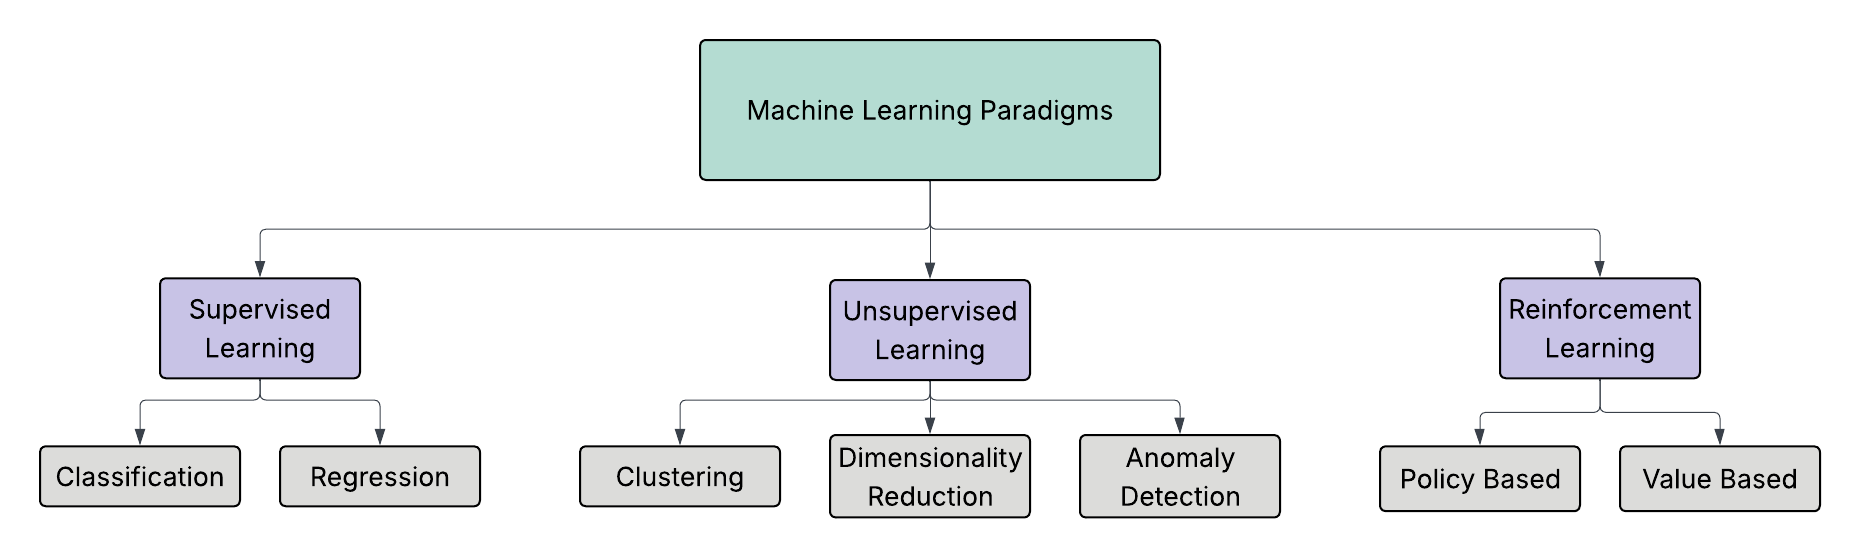
\includegraphics[width=0.9\textwidth]{Figures/ML-Paradigms.png}
    \caption{Overview of machine learning paradigms with common tasks.}
    \label{fig:ml_paradigms}
\end{figure}

\subsection{Selecting Machine Learning Method}